\documentclass[10pt,openany]{book}
\usepackage[top=2.25cm,bottom=1.75cm,left=1.5cm,right=1.5cm,headsep=5mm,letterpaper]{geometry}
\usepackage[spanish,es-noshorthands]{babel}
\usepackage{graphicx}
\usepackage[utf8]{inputenc}
\usepackage{float}

\usepackage{answers}
\usepackage{setspace}
\usepackage{enumitem}
\usepackage{multicol}
\usepackage{mathrsfs}
\usepackage{calligra}
\usepackage[usenames]{color}
\usepackage{amsmath,amsthm,amssymb}
\usepackage{esvect}
\usepackage{float}
\usepackage{geometry}
\geometry{left=25mm, right=14mm, top=10mm}
\usepackage[most]{tcolorbox}
\usepackage[hidelinks]{hyperref}
\usepackage{color}
\usepackage{subfig}
\usepackage[american]{circuitikz}
\usepackage{enumitem,amssymb}
\newlist{todolist}{itemize}{2}
\setlist[todolist]{label=$\square$}
\usepackage{cite} 

\usepackage{listings} % Paquete para código
\lstdefinelanguage{SQL}{
    keywords={SELECT, INSERT, UPDATE, DELETE, FROM, WHERE, JOIN, INNER, LEFT, RIGHT, ON, GROUP BY, ORDER BY, CREATE TABLE, PRIMARY KEY, FOREIGN KEY, REFERENCES, UNIQUE, NOT NULL, DEFAULT},
    sensitive=true,
    comment=[l]{--},
    morecomment=[s]{/*}{*/},
    string=[b]",
    morestring=[b]',
}

\def\rcurs{{\mbox{$\resizebox{.16in}{.08in}{\includegraphics{ScriptR}}$}}}
\def\brcurs{{\mbox{$\resizebox{.16in}{.08in}{\includegraphics{BoldR}}$}}}
\def\hrcurs{{\mbox{$\hat \brcurs$}}}

\newtcbtheorem{Problem}{\bfseries
Sección}{enhanced, drop shadow={black!50!white},
coltitle=black,
top=0.3in,
attach boxed title to top right={xshift=0em,yshift=-\tcboxedtitleheight/2},
boxed title style={size=small,colback=pink}}{summary}

\newcommand{\R}{\mathbb{R}}
\newcommand{\grad}{$^{\circ}$}
\renewcommand{\figurename}{{Figura}}

\DeclareMathOperator{\sech}{sech}
\DeclareMathOperator{\csch}{csch}

\begin{document}

\begin{titlepage}
\thispagestyle{empty}
\noindent
\begin{minipage}[c]{0.25\textwidth}%Primera columna

\begin{figure}[H]

\includegraphics[width=0.7\linewidth]{Figuras/Escudo-UNAM.pdf}
\end{figure}
\end{minipage}\hfill\begin{minipage}[c]{0.75\textwidth}%Segunda columna
\begin{center}
\textbf{\Huge {UNIVERSIDAD NACIONAL\\[2mm]
AUTÓNOMA DE MÉXICO}}\vspace{5mm}
\hrule height 2.5pt \vspace{5mm}
\textbf{\Huge {FACULTAD DE INGENIERÍA}}
\end{center}
\end{minipage}

\noindent
\begin{minipage}[t]{0.25\textwidth}%Primera columna
\vspace{5mm}
\hspace{0.9cm}
\vrule width2.5pt height13cm
\hspace{8mm}
\vrule width2.5pt height13cm
\end{minipage}\hfill\begin{minipage}[t]{0.75\textwidth}%Segunda columna

\begin{center}
\vspace{1cm}
\textbf{\huge {División de Ingeniería Eléctrica\\[2mm]
Departamento de Ingeniería en Computación}}\\[1.5cm]

\textbf{\huge {Bases de Datos}}\\[6mm]
\textbf{\LARGE {Proyecto final de la asignatura\\ de bases de datos}}\\[10mm]
\textbf{\LARGE {Ing. Fernando Arreola}}\\[10mm]
\textbf{\LARGE {Noviembre 2024}}\\[10mm]
\textbf{\LARGE {Equipo DataBenders:}}\\[6mm]
\textbf{\LARGE {Integrantes:}}\\[6mm]
\textbf{\LARGE {Luis Fernando Franco Arellano}}\\
\textbf{\LARGE {Gustavo Isaac Soto Huerta}}\\
\textbf{\LARGE {Eduardo Zavala Sánchez}}\\
\textbf{\LARGE {José Eduardo Villeda Tlecuitl}}
\end{center}
\end{minipage}
\noindent
\begin{minipage}[T]{0.25\textwidth}%Primera columna
\begin{figure}[H]

\includegraphics[width=0.7\linewidth]{Figuras/Ingenieria.jpg}
\end{figure}
\end{minipage}\hfill\begin{minipage}[c]{0.75\textwidth}%Segunda columna
\vspace{2cm}
\textbf{Semestre 2025 - 1} \hfill \textbf{Fecha de realización: 23 de Agosto de 2024}
\end{minipage}
\end{titlepage}

\pagebreak


\chapter{Introducción}

En el ámbito de la gestión empresarial, el manejo adecuado y eficiente de la información es fundamental para optimizar procesos y mejorar la toma de decisiones. Este proyecto tiene como propósito desarrollar una solución de base de datos que permita a una cadena de papelerías almacenar y organizar su información de forma estructurada y accesible, contribuyendo así a su modernización operativa. La implementación de esta base de datos busca satisfacer una serie de requerimientos específicos, tales como el almacenamiento de datos detallados de proveedores, clientes, inventarios y transacciones de ventas, asegurando a su vez la integridad de la información y la eficiencia en su manejo.

Este sistema no sólo se limita a almacenar información; también está diseñado para automatizar ciertos procesos críticos, como la generación de facturas, la actualización del inventario, y el cálculo de utilidades, entre otros. A lo largo del desarrollo, se deberán aplicar conceptos de diseño de bases de datos y lenguajes de consulta, tomando en cuenta las particularidades del negocio y las reglas de integridad que garanticen la consistencia de los datos. Además, se realizarán configuraciones específicas, tales como la creación de índices y estructuras adicionales para optimizar el acceso a la información y la generación de reportes.

De este modo, el proyecto permite a los estudiantes aplicar conocimientos de diseño y administración de bases de datos en un contexto práctico, explorando cómo una infraestructura de datos bien construida puede ofrecer un soporte fundamental a las operaciones y la estrategia de una empresa.

\section{Objetivo}
El alumno analizará una serie de requerimientos y propondrá una solución que atienda a los mismos, aplicando los conceptos vistos en el curso.

\section{Descripción del Problema}
El problema se divide en dos partes:

\subsection{Parte Uno}
Consiste en el diseño de una base de datos. Una cadena de papelerías busca innovar la manera en que almacena su información, y los contratan para que desarrollen los sistemas informáticos para satisfacer los siguientes requerimientos:

\begin{itemize}
    \item Se desea tener almacenados datos como la razón social, domicilio, nombre y teléfonos de los proveedores; RFC, nombre, domicilio y al menos un email de los clientes.
    \item Es necesario tener un inventario de los productos que se venden, en el que debe guardarse el código de barras, precio al que fue comprado el producto, foto, fecha de compra y cantidad de ejemplares en la bodega (stock).
    \item Se desea guardar la marca, descripción y precio de los regalos, artículos de papelería, impresiones y recargas, siempre y cuando se tenga su correspondiente registro en el inventario.
    \item Debe también guardarse el número de venta, fecha de venta, la cantidad total a pagar por la venta, empleado que concreta la venta, así como la cantidad de cada artículo y precio total a pagar por artículo.
    \item De los empleados interesa conocer su clave de empleado, nombre, fecha de nacimiento y fecha de ingreso.
\end{itemize}

Adicional al almacenamiento de información, se requiere que el sistema resuelva lo siguiente:

\begin{itemize}
    \item Cada que se solicite, se genere una muestra de información que contenga la información necesaria para asemejarse a una factura de una compra.
    \item Dada una fecha, o una fecha de inicio y fecha de fin, regresar la cantidad total que se vendió y la ganancia correspondiente en esa fecha o periodo.
    \item Cada que haya la venta de un artículo, deberá decrementarse el stock por la cantidad vendida de ese artículo. Si el valor llega a cero, abortar la transacción. Si el pedido se completa pero quedan menos de 3 en stock, se deberá emitir una alerta. Debe actualizarse el total a pagar por artículo y el total a pagar por la venta.
    \item Permitir obtener el nombre de aquellos productos de los cuales hay menos de 3 en stock. El resultado debe almacenarse en una tabla independiente que sólo debe almacenar la información actualizada.
    \item Al recibir el código de barras de un producto, regrese la utilidad.
    \item Crear al menos un índice, del tipo que se prefiera y donde se prefiera. Justificar el porqué de la elección en ambos aspectos.
\end{itemize}

\subsection{Consideraciones}
\begin{itemize}
    \item Puede haber distintas soluciones al problema.
    \item Los requerimientos enlistados anteriormente deberán ser realizados por medio de PgSQL, con los elementos que se consideren adecuados para resolverlos.
    \item El folio de la venta debe tener un formato similar a VENT-001, prefijo \texttt{VENT}, seguido de un guion y un número secuencial.
    \item Donde esté presente el atributo \texttt{domicilio}, está compuesto por estado, código postal, colonia, calle y número.
    \item Donde esté presente el atributo \texttt{nombre}, está compuesto por nombre, apellido paterno y materno.
    \item La propuesta debe contemplar todas las etapas de diseño, las consideraciones anteriores y un buen manejo de información.
\end{itemize}

\subsection{Parte dos}
Una vez diseñada e implementada la base de datos, deberá elegirse la integración de alguno de los siguientes puntos:
\begin{enumerate}
    \item Generar un dashboard que permita visualizar, al menos:
    \begin{itemize}
        \item Ingresos del mes (Invertido, Ingresos y Ganancias)
        \item Top 3 de artículos más vendidos
        \item Empleados que registran más órdenes
    \end{itemize}
    \item Programar en C o en Java, un objeto que simule ser una tabla de una base de datos, lo que implica que permita ingresar, borrar, actualizar y consultar información.
    \item Ingresar, a partir de archivos de texto, la información registrada durante el día a otra base de datos. Se debe orquestar la inserción de cada archivo y tener validaciones del flujo en caso de errores.
\end{enumerate}

\subsection{Entregables}
Es necesario entregar lo que se solicita a continuación:

\subsection{Documento}
Se deberá entregar un documento \textbf{FORMAL} elaborado en LaTeX, que contenga las siguientes secciones:
\begin{itemize}
    \item \textbf{Introducción:} Breve descripción del análisis del problema, sus objetivos, su(s) propuesta(s) de solución. Elaborada por ustedes mismos.
    \item \textbf{Plan de trabajo:} Queda a criterio de cada equipo el grado de detalle que se le dará a esta sección, pero mínimo debe contener descripción general de las actividades a realizar, su correspondiente plan de actividades y un breve detalle de qué hizo cada miembro del equipo.
    \item \textbf{Diseño:} Descripción de lo realizado en las correspondientes fases de diseño de las bases de datos, agregando los resultados de cada una de ellas.
    \item \textbf{Implementación:} Descripción de funcionamiento y código de los \textit{stored procedures}, \textit{triggers}, funciones, etc. empleados para cumplir con los requerimientos del problema. También debe incluirse el DDL de la base de datos.
    \item \textbf{Presentación:} Descripción de lo que hace la modalidad seleccionada como forma de conexión hacia la base de datos.
    \item \textbf{Conclusiones:} Personales, detallando las dificultades, retos, aciertos, etc. que se presentaron en el proyecto.
\end{itemize}

\subsection{Código}
A través de GitHub, se deberá crear una carpeta por equipo donde se anexe lo siguiente, asignando nombres \textbf{ADECUADOS} para cada documento/archivo:
\begin{itemize}
    \item El documento del punto anterior
    \item Códigos fuente de MER, MR
    \item Script de creación de la base de datos y tablas
    \item Script para el agregado de información
    \item Script de toda la programación a nivel BD
    \item Códigos de lo implementado como parte de la etapa de presentación
    \item La presentación a emplear a la hora de exponer
\end{itemize}

\section{Exposición}
Como parte de la evaluación del curso, se deberá realizar una presentación del proyecto. La idea es simular la presentación de una solución de software a un posible cliente, lo que implica descripción del software, muestras de funcionalidad, solución de dudas, etc. Cada equipo es libre de decidir cómo hacer su presentación, el único detalle es que debe ser \textbf{TOTALMENTE formal}.

\section{Puntos a considerar}
Se tomará en cuenta lo siguiente, partiendo del porcentaje de calificación estipulado al inicio del semestre:
\begin{itemize}
    \item Equipos que se copien en alguna parte del proyecto, su calificación del curso será 5.
    \item Equipo(s) que reprueben el proyecto o la parte de exposición, deberán presentar examen final sin importar lo obtenido en los otros rubros del curso.
    \item La calificación del primer examen final será 30\% lo obtenido en el proyecto, 70\% lo obtenido en el examen.
    \item La seriedad, formalidad, presentación y calidad del proyecto, si bien no tendrán un valor numérico específico, pueden jugar a favor o en contra de la calificación de los rubros correspondientes.
    \item Cualquier punto no contemplado en el presente documento será determinado por el profesor.
\end{itemize}

\section{Recomendaciones}
No es obligatorio, pero se sugieren los siguientes puntos:
\begin{itemize}
    \item Delegar correctamente responsabilidades
    \item No demorar en formar sus equipos y agregar su carpeta en GitHub
    \item Empleo de herramientas colaborativas
    \item Empleo de arquitecturas cliente-servidor remotas o servicios en la nube
    \item Redacción y presentación en inglés
\end{itemize}


\chapter{Desarrollo de la Parte Uno}

\section{Entidades, Atributos y Relaciones Encontradas}

Esta sección presenta el Modelo Entidad-Relación (MER) correspondiente al sistema de gestión de la cadena de tiendas de papelería. A continuación se describen las entidades, sus atributos y las relaciones que se han identificado para cumplir con los requerimientos del sistema.

\subsection{Entidades y Atributos}

Para desarrollar este modelo, identificamos 10 entidades clave. Decidimos incorporar catálogos individuales para estados y países, lo cual facilita tanto la búsqueda como la inserción de datos en el sistema. Esto permite mantener la consistencia de datos al gestionar ubicaciones.

En cuanto a las relaciones, solo se identificó una entidad débil: \textbf{StockBajo}. Esta entidad es débil porque depende exclusivamente de la existencia de un producto.

A continuación, se detallan las entidades principales junto con sus atributos:

\begin{itemize}
    \item \textbf{Proveedores}
        \begin{itemize}
            \item \textbf{ProveedorID} (Clave Primaria)
            \item NombreComercial
            \item Domicilio
            \begin{itemize}
                \item Domicilio\_Calle
                \item Domicilio\_Número
                \item Domicilio\_Colonia
                \item Domicilio\_CódigoPostal
                \item Domicilio\_Estado
            \end{itemize}
            \item Nombre
            \begin{itemize}
                \item Nombre
                \item ApellidoPaterno
                \item ApellidoMaterno (Opcional)
            \end{itemize}
            \item Teléfonos (Multivalorado)
            \item RFC (Clave Candidata)
        \end{itemize}
        
    \item \textbf{Clientes}
        \begin{itemize}
            \item \textbf{ClienteID} (Clave Primaria)
            \item Nombre
            \begin{itemize}
                \item Nombre
                \item ApellidoPaterno
                \item ApellidoMaterno (Opcional)
            \end{itemize}
            \item Domicilio
            \begin{itemize}
                \item Domicilio\_Calle
                \item Domicilio\_Número
                \item Domicilio\_Colonia
                \item Domicilio\_CódigoPostal
                \item Domicilio\_Estado
            \end{itemize}
            \item CorreosElectrónicos (Multivalorado)
            \item RFC (Clave Candidata) (Opcional)
        \end{itemize}
        
    \item \textbf{Productos}
        \begin{itemize}
            \item \textbf{ProductoID} (Clave Primaria)
            \item CódigoBarras (Clave Candidata)
            \item Nombre
            \item PrecioCompra
            \item PrecioVenta
            \item Foto
            \item CantidadStock
        \end{itemize}
        
    \item \textbf{Categorías}
        \begin{itemize}
            \item \textbf{CategoríaID} (Clave Primaria)
            \item Nombre
            \item Descripción
        \end{itemize}
        
    \item \textbf{Ventas}
        \begin{itemize}
            \item \textbf{VentaID} (Clave Primaria)
            \item Folio (Clave Candidata)
            \item FechaVenta
            \item MontoTotalPagar
        \end{itemize}
        
    \item \textbf{Empleados}
        \begin{itemize}
            \item \textbf{EmpleadoID} (Clave Primaria)
            \begin{itemize}
                \item Nombre
                \item ApellidoPaterno
                \item ApellidoMaterno (Opcional)
            \end{itemize}
            \item FechaNacimiento
            \item FechaIngreso
        \end{itemize}
        
    \item \textbf{Producto\_Venta} (Relación)
        \begin{itemize}
            \item CantidadProducto
            \item PrecioTotalProducto
        \end{itemize}
        
    \item \textbf{StockBajo}
        \begin{itemize}
            \item \textbf{ProductoID} (Clave Primaria)
            \item EsStockBajo
        \end{itemize}
        
    \item \textbf{Países}
        \begin{itemize}
            \item \textbf{PaísID} (Clave Primaria)
            \item Nombre
        \end{itemize}
        
    \item \textbf{Estados}
        \begin{itemize}
            \item \textbf{EstadoID} (Clave Primaria)
            \item Nombre
        \end{itemize}
\end{itemize}


\subsection{Relaciones}

\begin{itemize}
    \item \textbf{Proveedor} a \textbf{Producto:} Un proveedor puede ofrecer múltiples productos (1:M).
    \item \textbf{Cliente} a \textbf{Venta:} Un cliente puede realizar múltiples ventas (1:M).
    \item \textbf{Venta} a \textbf{Producto:} Muchos productos pueden estar contenidos en muchas ventas (M:M). Esta relación puede tener atributos adicionales, como \textit{Cantidad} y \textit{PrecioTotal}.
    \item \textbf{Categoría} a \textbf{Producto:} Cada producto pertenece a una categoría (M:1).
    \item \textbf{Empleado} a \textbf{Venta:} Un empleado puede registrar múltiples ventas (1:M).
    \item \textbf{Estado} a \textbf{Cliente:} Un cliente reside en un estado (1:M).
    \item \textbf{Estado} a \textbf{Proveedor:} Un proveedor reside en un estado (1:M).
    \item \textbf{País} a \textbf{Estado:} Un estado pertenece a un país (1:M).
    \item \textbf{Cliente} a \textbf{CorreosElectrónicosCliente:} Un cliente puede tener múltiples direcciones de correo electrónico (1:M).
\end{itemize}


\section{Modelo Entidad-Relación}

\begin{figure}[H]
    \begin{center}
        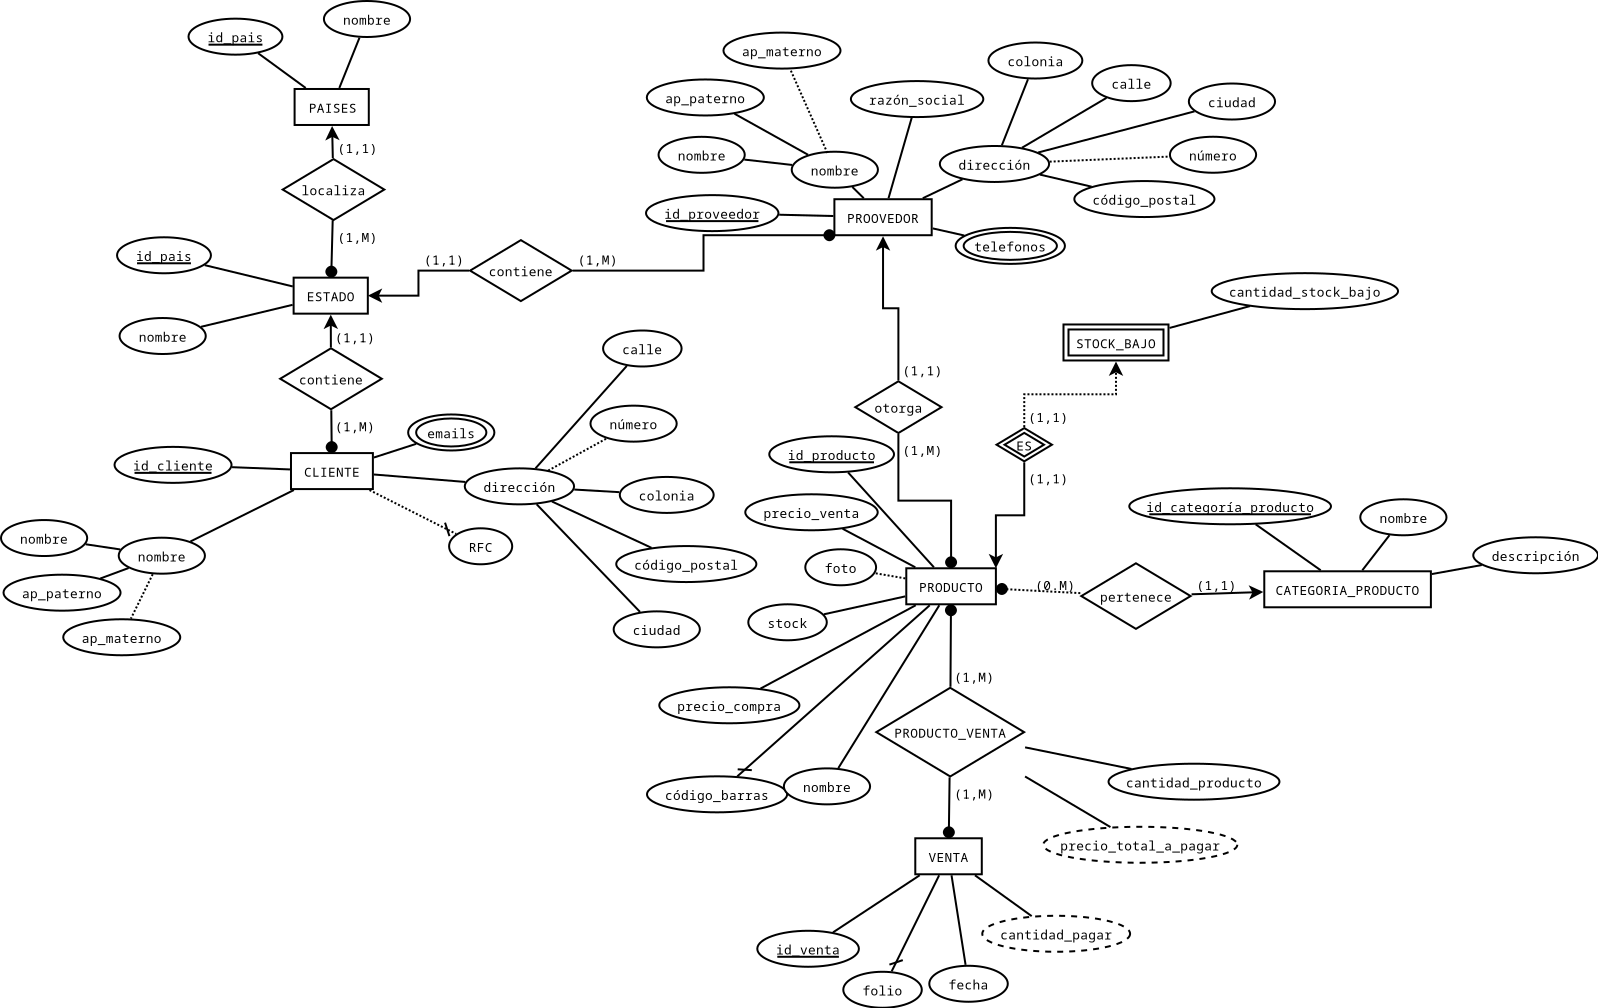
\includegraphics[width=\textwidth]{Imagenes/modelo_ER.png}
        \caption{Modelo Entidad-Relación de nuestro caso de estudio}
    \end{center}
\end{figure}

\section{Entidades, atributos y relaciones en modelo relacional}

Basamos nuestra representación en las recomendaciones de la documentación de PGModeler \nocite{pgModeler_Relationships}, donde revisamos cómo representar nuestro caso de estudio en el modelo relacional.

\begin{itemize}
    \item \textbf{Proveedores}
        \begin{itemize}
            \item \textbf{ProveedorID} (PK)
            \item RazonSocial (VARCHAR(100))
            \item Domicilio
            \begin{itemize}
                \item Domicilio\_Calle (VARCHAR(100))
                \item Domicilio\_Numero (VARCHAR(10))
                \item Domicilio\_Colonia (VARCHAR(100))
                \item Domicilio\_CodigoPostal (VARCHAR(10))
                \item Domicilio\_EstadoID (FK)
            \end{itemize}
            \item Nombre (VARCHAR(100))
            \item RFC (VARCHAR(50), Unique)
        \end{itemize}
        
    \item \textbf{ProveedorTelefonos}
        \begin{itemize}
            \item \textbf{TelefonoID} (PK)
            \item ProveedorID (FK)
            \item NumeroTelefono (VARCHAR(20))
            \item TipoTelefono (VARCHAR(50)) % Ejemplo: 'Móvil', 'Oficina', 'Fax', etc.
        \end{itemize}
        
    \item \textbf{Clientes}
        \begin{itemize}
            \item \textbf{ClienteID} (PK)
            \item Nombre (VARCHAR(100))
            \item ApellidoPaterno (VARCHAR(100))
            \item ApellidoMaterno (VARCHAR(100))
            \item Domicilio
            \begin{itemize}
                \item Domicilio\_Calle (VARCHAR(100))
                \item Domicilio\_Numero (VARCHAR(10))
                \item Domicilio\_Colonia (VARCHAR(100))
                \item Domicilio\_CodigoPostal (VARCHAR(10))
                \item Domicilio\_EstadoID (FK)
            \end{itemize}
            \item Emails (VARCHAR(100), Multivaluado)
            \item RFC (VARCHAR(50), Unique) (NULL)
        \end{itemize}
        
    \item \textbf{Productos}
        \begin{itemize}
            \item \textbf{ProductoID} (PK)
            \item CodigoBarras (VARCHAR(50), UNIQUE)
            \item Nombre (VARCHAR(100))
            \item PrecioCompra (DECIMAL(10, 2))
            \item PrecioVenta (DECIMAL(10, 2))
            \item Foto (BLOB)
            \item CantidadStock (INT)
            \item CategoriaID (FK)
            \item ProveedorID (FK)
        \end{itemize}
        
    \item \textbf{Categorias}
        \begin{itemize}
            \item \textbf{CategoriaID} (PK)
            \item Nombre (VARCHAR(100))
            \item Descripcion (TEXT)
        \end{itemize}
        
    \item \textbf{Ventas}
        \begin{itemize}
            \item \textbf{VentaID} (PK)
            \item Folio (VARCHAR(20), Unique)
            \item FechaVenta (DATE)
            \item CantidadTotalPagar (NUMERIC(10, 2))
            \item EmpleadoID (FK)
        \end{itemize}
        
    \item \textbf{Empleados}
        \begin{itemize}
            \item \textbf{EmpleadoID} (PK)
            \item Nombre (VARCHAR(100))
            \item ApellidoPaterno (VARCHAR(100))
            \item ApellidoMaterno (VARCHAR(100))
            \item FechaNacimiento (DATE)
            \item FechaIngreso (DATE)
        \end{itemize}
        
    \item \textbf{DetalleVenta}
        \begin{itemize}
            \item \textbf{DetalleVentaID} (PK)
            \item VentaID (FK)
            \item ProductoID (FK)
            \item CantidadProducto (INT)
            \item PrecioTotalArticulo (NUMERIC(10, 2))
        \end{itemize}
        
    \item \textbf{StockBajo}
        \begin{itemize}
            \item \textbf{ProductoID} (PK, FK)
            \item EnBajoStock (BOOLEAN, DEFAULT FALSE)
        \end{itemize}
        
    \item \textbf{Paises}
        \begin{itemize}
            \item \textbf{PaisID} (PK)
            \item Nombre (VARCHAR(100))
        \end{itemize}
        
    \item \textbf{Estados}
        \begin{itemize}
            \item \textbf{EstadoID} (PK)
            \item Nombre (VARCHAR(100))
            \item PaisID (FK)
        \end{itemize}
        
    \item \textbf{ClienteEmails}
        \begin{itemize}
            \item ClienteID (FK)
            \item Email (VARCHAR(100))
            \item \textbf{PRIMARY KEY (ClienteID, Email)}
        \end{itemize}
\end{itemize}

\section{Modelo Relacional}

\begin{figure}[H]
    \begin{center}
        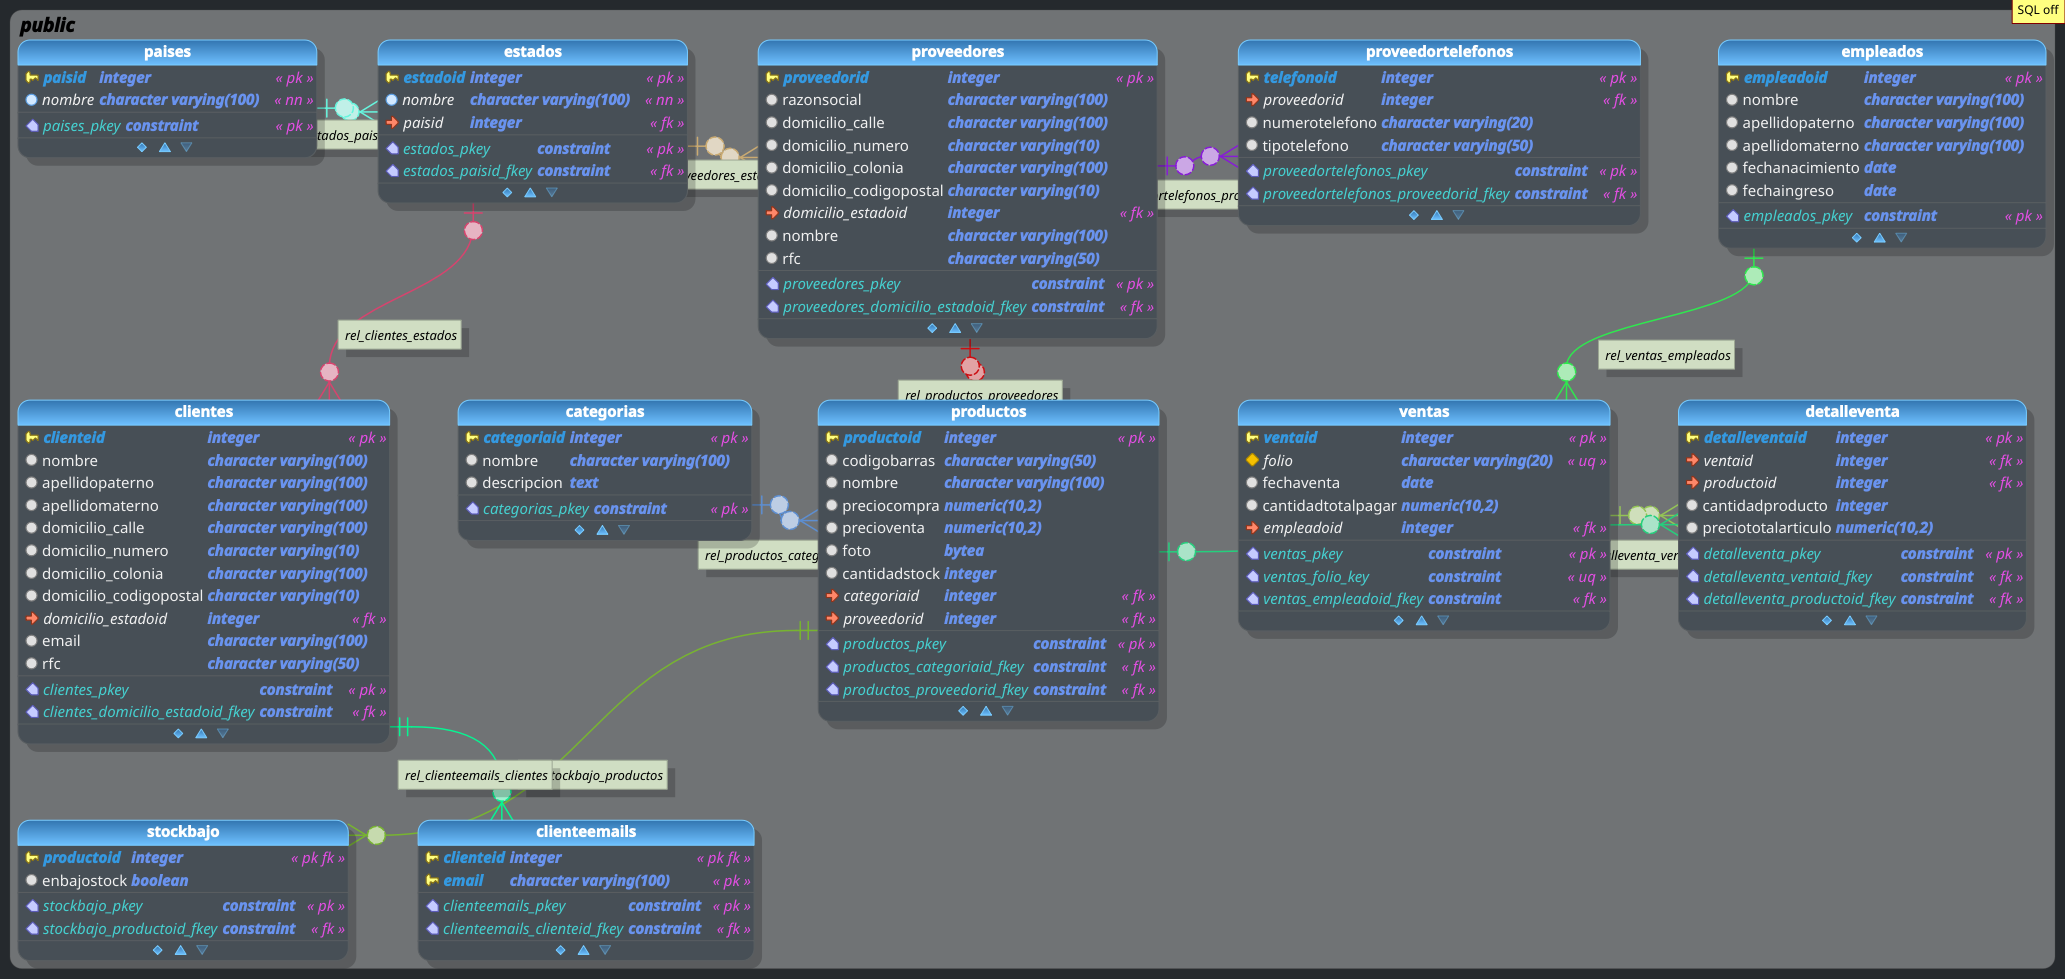
\includegraphics[width=\textwidth]{Imagenes/modelo_R.png}
        \caption{Modelo relacional de nuestro modelo}
    \end{center}
\end{figure}


\section{Desarrollo del modelo físico}

Basandonos en nuestro modelo relacional generamos el siguiente código SQL con la herramienta PGModeler y en la documentación del desarollo de sentencias SQL para PostgreSQL \nocite{PostgreSQL_DDL}obtuvimos el siguiente modelo físico.


\begin{lstlisting}[language=SQL]
CREATE TABLE Paises (
    PaisID INT PRIMARY KEY GENERATED BY DEFAULT AS IDENTITY,
    Nombre VARCHAR(100) NOT NULL
);

CREATE TABLE Estados (
    EstadoID INT PRIMARY KEY GENERATED BY DEFAULT AS IDENTITY,
    Nombre VARCHAR(100) NOT NULL,
    PaisID INT,
    FOREIGN KEY (PaisID) REFERENCES Paises(PaisID)
);

CREATE TABLE Proveedores (
    ProveedorID INT PRIMARY KEY GENERATED BY DEFAULT AS IDENTITY,
    RazonSocial VARCHAR(100),
    Domicilio_Calle VARCHAR(100),
    Domicilio_Numero VARCHAR(10),
    Domicilio_Colonia VARCHAR(100),
    Domicilio_CodigoPostal VARCHAR(10),
    Domicilio_EstadoID INT,
    Nombre VARCHAR(100),
    RFC VARCHAR(50),
    FOREIGN KEY (Domicilio_EstadoID) REFERENCES Estados(EstadoID)
);

CREATE TABLE ProveedorTelefonos (
    TelefonoID INT PRIMARY KEY GENERATED BY DEFAULT AS IDENTITY,
    ProveedorID INT,
    NumeroTelefono VARCHAR(20),
    TipoTelefono VARCHAR(50), -- Ejemplo: 'Móvil', 'Oficina', 'Fax', etc.
    FOREIGN KEY (ProveedorID) REFERENCES Proveedores(ProveedorID)
);

CREATE TABLE Empleados (
    EmpleadoID INT PRIMARY KEY GENERATED BY DEFAULT AS IDENTITY,
    Nombre VARCHAR(100),
    ApellidoPaterno VARCHAR(100),
    ApellidoMaterno VARCHAR(100),
    FechaNacimiento DATE,
    FechaIngreso DATE
);

CREATE TABLE Clientes (
    ClienteID INT PRIMARY KEY GENERATED BY DEFAULT AS IDENTITY,
    Nombre VARCHAR(100),
    ApellidoPaterno VARCHAR(100),
    ApellidoMaterno VARCHAR(100),
    Domicilio_Calle VARCHAR(100),
    Domicilio_Numero VARCHAR(10),
    Domicilio_Colonia VARCHAR(100),
    Domicilio_CodigoPostal VARCHAR(10),
    Domicilio_EstadoID INT,
    Email VARCHAR(100),
    RFC VARCHAR(50),
    FOREIGN KEY (Domicilio_EstadoID) REFERENCES Estados(EstadoID)
);

CREATE TABLE Categorias (
    CategoriaID INT PRIMARY KEY GENERATED BY DEFAULT AS IDENTITY,
    Nombre VARCHAR(100),
    Descripcion TEXT
);

CREATE TABLE Productos (
    ProductoID INT PRIMARY KEY GENERATED BY DEFAULT AS IDENTITY,
    CodigoBarras VARCHAR(50),
    Nombre VARCHAR(100),
    PrecioCompra DECIMAL(10, 2),
    PrecioVenta DECIMAL(10, 2),
    Foto BYTEA,
    CantidadStock INT,
    CategoriaID INT,
    ProveedorID INT,
    FOREIGN KEY (CategoriaID) REFERENCES Categorias(CategoriaID),
    FOREIGN KEY (ProveedorID) REFERENCES Proveedores(ProveedorID)
);

CREATE TABLE Ventas (
    VentaID INT PRIMARY KEY GENERATED BY DEFAULT AS IDENTITY,
    Folio VARCHAR(20) UNIQUE,
    FechaVenta DATE,
    CantidadTotalPagar DECIMAL(10, 2),
    EmpleadoID INT,
    FOREIGN KEY (EmpleadoID) REFERENCES Empleados(EmpleadoID)
);

CREATE TABLE DetalleVenta (
    DetalleVentaID INT PRIMARY KEY GENERATED BY DEFAULT AS IDENTITY,
    VentaID INT,
    ProductoID INT,
    CantidadProducto INT,
    PrecioTotalArticulo DECIMAL(10, 2),
    FOREIGN KEY (VentaID) REFERENCES Ventas(VentaID),
    FOREIGN KEY (ProductoID) REFERENCES Productos(ProductoID)
);

CREATE TABLE StockBajo (
    ProductoID INT PRIMARY KEY,
    EnBajoStock BOOLEAN DEFAULT FALSE,
    FOREIGN KEY (ProductoID) REFERENCES Productos(ProductoID)
);

CREATE TABLE ClienteEmails (
    ClienteID INT,
    Email VARCHAR(100),
    PRIMARY KEY (ClienteID, Email),
    FOREIGN KEY (ClienteID) REFERENCES Clientes(ClienteID)
);
\end{lstlisting}


\bibliographystyle{apalike}
\bibliography{ref}

\end{document}
